\chapter{Architecture and implementation}

The application is divided into three parts:
	\begin{itemize}
		\addtolength{\itemindent}{1cm}
		\item The Neuronal Network Engine
		\item The User Input Handling and Processing
		\item The Application-User interaction via the GUI
	\end{itemize}

We will continue this chapter by entering into the details of each of the aforementioned component.

\section{The Neuronal Network Engine}

The Neural Network Engine was developed using the Neural Network Framework which we implemented from scratch. The
Neural Network Framework contains various tools for Neural Network problem solving such as layers, optimizers, metrics,
etc. The Neural Network Framework operates a \textit{model} file, a binary serialized file which supports the following
operations:
	\begin{itemize}
		\item Training: Initializing/improving the performance by performing predictions over a given input
			data in order to adjust the \textit{weights and biases} (the model \textit{neurons}).
		\item Inference: Performing predictions over unseen data.
		\item Loading: Loading a previously trained model in order to perform inference/ continue the training process
		\item Saving: Creating/writing the results of the previous operations.

	\end{itemize}
The main application problem can be reduced to a binary classification problem ( the engine has to predict if a given
input falls into the category Piano or Other), thus we choosen the following architecture:


\begin{figure}[H]
	\centering
	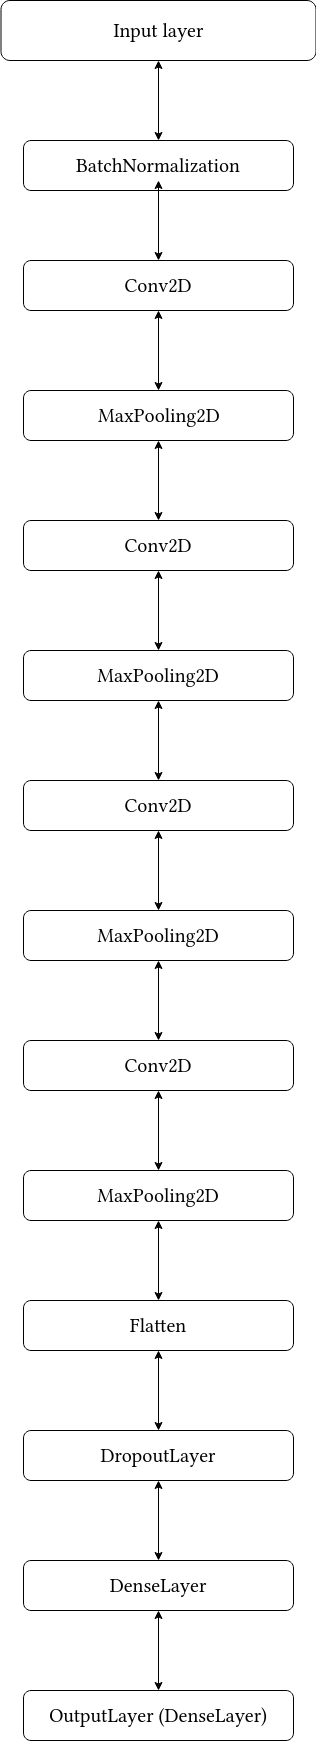
\includegraphics[width = 1.5in]{images/summary.png}
	\caption{A summary of the model architecture}
\label{model_arch}
\end{figure}

The model is composed of layers, which fall into two categories: trainable (Conv2D, MaxPooling2D, DenseLayer), and non-trainable
(InputLayer, FlattenLayer, DropoutLayer, BatchNormalization). The difference between the two categories is the type of the operations
performed, and whether or not they facilitate the learning process.\\

For the trainable layers we choosen the \textit{Adam}(Adaptive Moment estimation) optimizer, which works
by combining the \textit{Adagrad} and \textit{RMSProp} optimizers by calculating an exponential moving average
of the gradient and the squared gradient, as well as controling the decay rates of these moving averages.\cite{nnfs}

The activation function we had choosen for the trainable layers is \textit{ReLU}(Rectified Linear Unit), while for
the activation layer we preferred the \textit{SoftmaxActivation} because, unlike linear activation functions,
the aforemetioned activation function returns the probability values normalized between 0 and 1, handling
very small negative or exploding values by penalizing them.


The metrics measured throughout the learning process are computed using \textit{CategoricalAccuracy} and
\textit{CategoricalCrossentropy}.




The Neural Network Engine consists of a trained model, containing the weights and biases of the trainable layers from
the figure \ref{model_arch}.

The model values and its performance are the result of the training process, which consisted of five epochs over 33602
inputs values (one second wav audio snippets), presented to the model in the form of \textit{batches} provided
by the custom \textit{Data generator}, with each batch containing 32 samples. The batch size as well as other
configuration parameters (e.g. \textit{filter shape, pool size, dropout rate}) are arbitrary values choosen
after performing the \textit{fine tuning} phase of the training, which consists of repeatedly training models with
different configurations (also known as \textit{hyperparameter adjusting}), in order to obtain an optimal configuration.


The data was gathered by web scraping various YouTube playlists using the \textit{youtube-dl} utilitary, obtaining a
diverse and feature rich dataset.
The "Piano" category consists of isolated tracks which only contain piano snippets(any other combination of instruments
will not be classified as expected by the model), while the "Other" category contains every other category of sounds.

The distribution of the data is presented in the below figure:

\begin{center}
	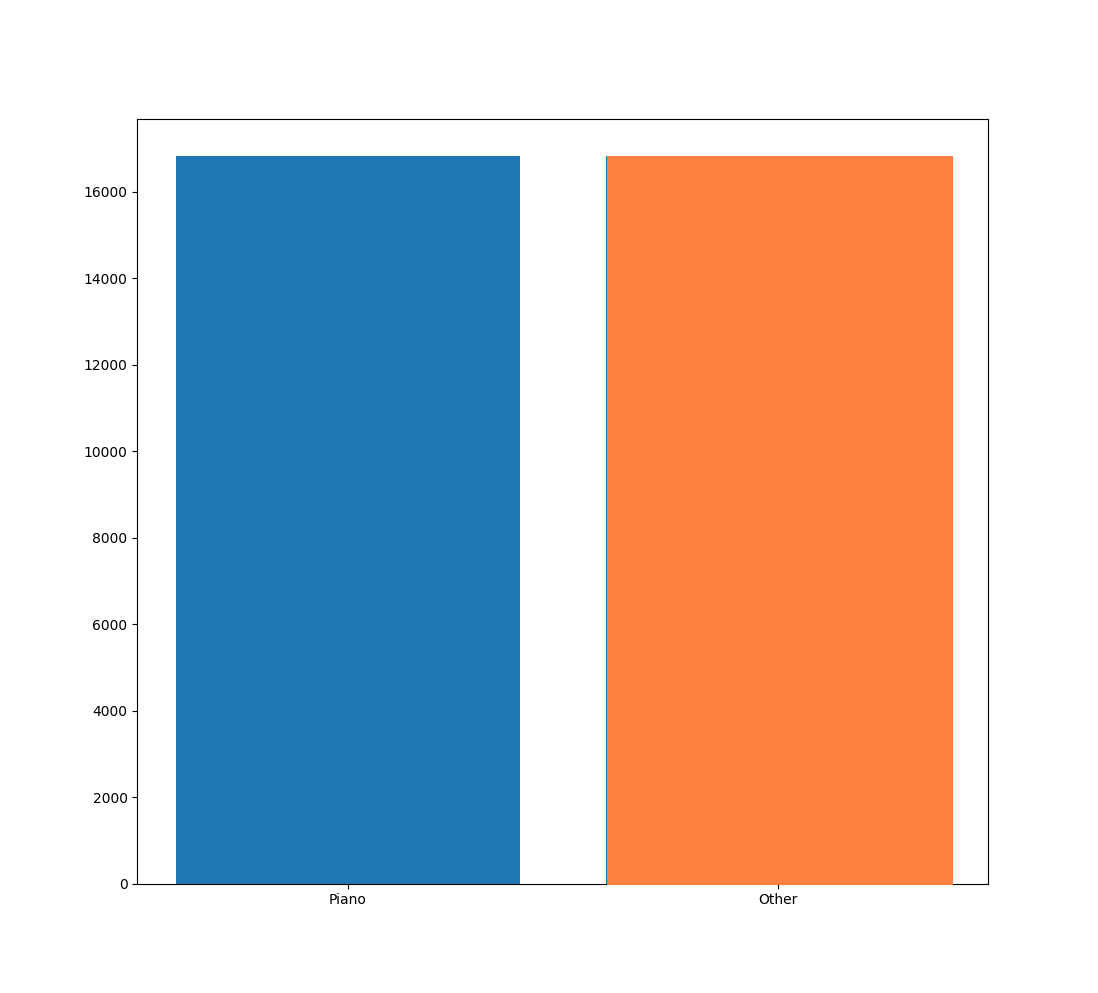
\includegraphics[width = 4.2in]{images/datadistr.png}
	\centerline{\captionof{Figure 4.2: }{Data distribution by number of samples.}}
\label{dd}
\end{center}

Initially we approached the problem without using Convolutional Operations, but after testing numerous configurations
the results were below satisfying (with the loss stagnating at a value of about 0.5 ) and the accuracy fluctuating between 40-60\%, as ilustrated in the figures below.


\begin{center}
	\centering
	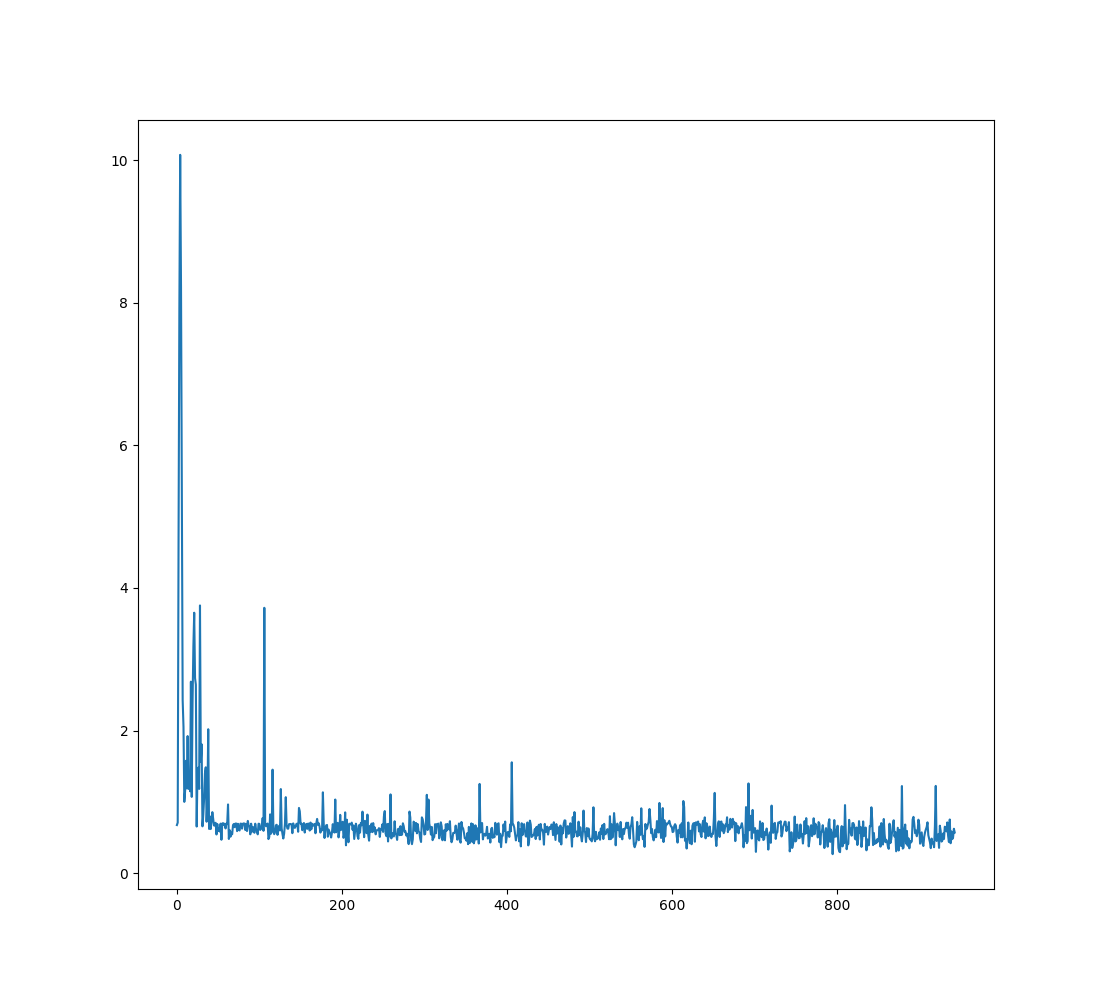
\includegraphics[width = 4.2in]{images/badmetricspng.png}
	\centerline{\captionof{Figure 4.3: }{Model loss before adding Convolutional Operations to the Model}}
\label{bad_metrics}
\end{center}


\begin{center}
	\centering
	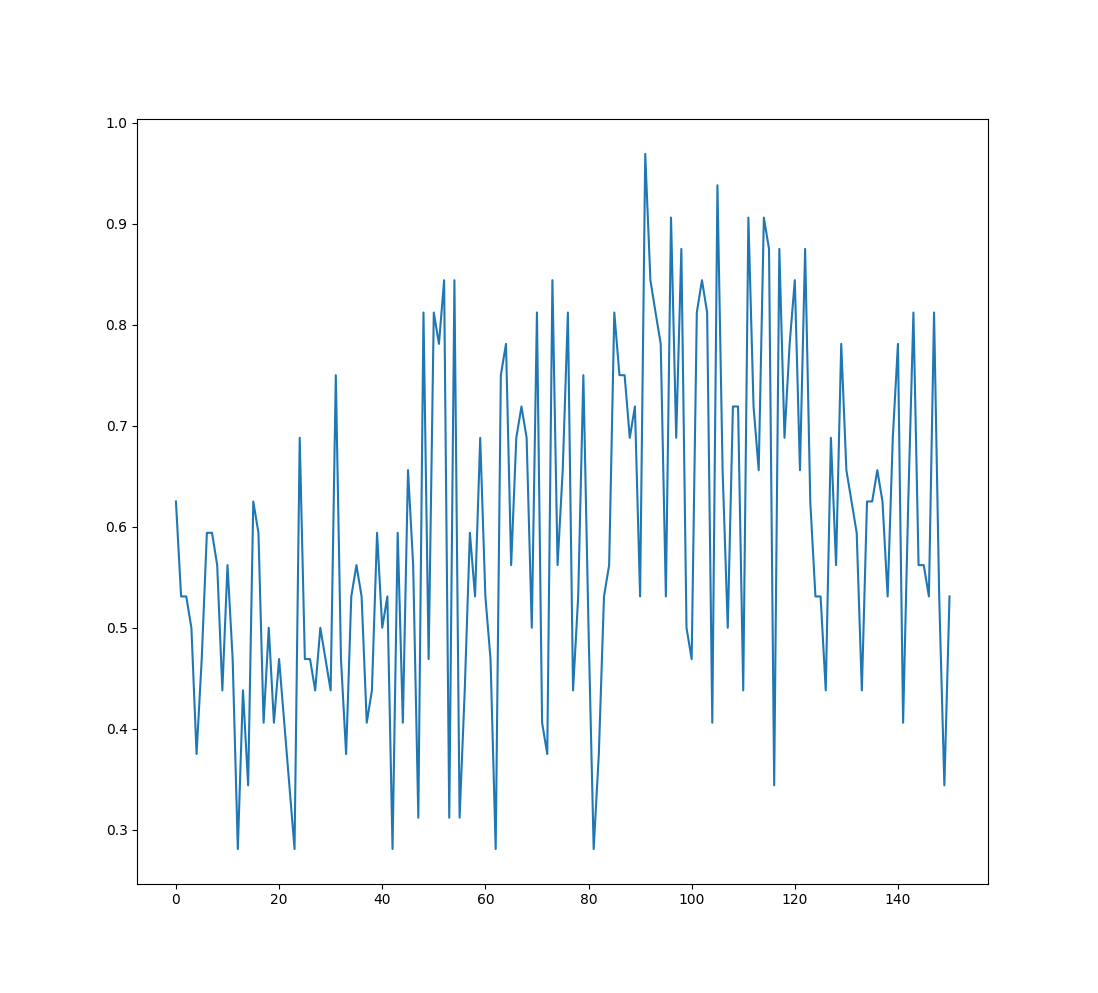
\includegraphics[width = 4.2in]{images/badacc.png}
	\centerline{\captionof{Figure 4.4: }{Model accuracy before adding Convolutional Operations to the Model}}
\label{bad_metrics2}
\end{center}
By incorporating the Convolutional Operations and Layers into the Neural Network Framework, the model accuracy as well
as the loss improved at a visible rate, as shown below.


\begin{center}
	\centering
	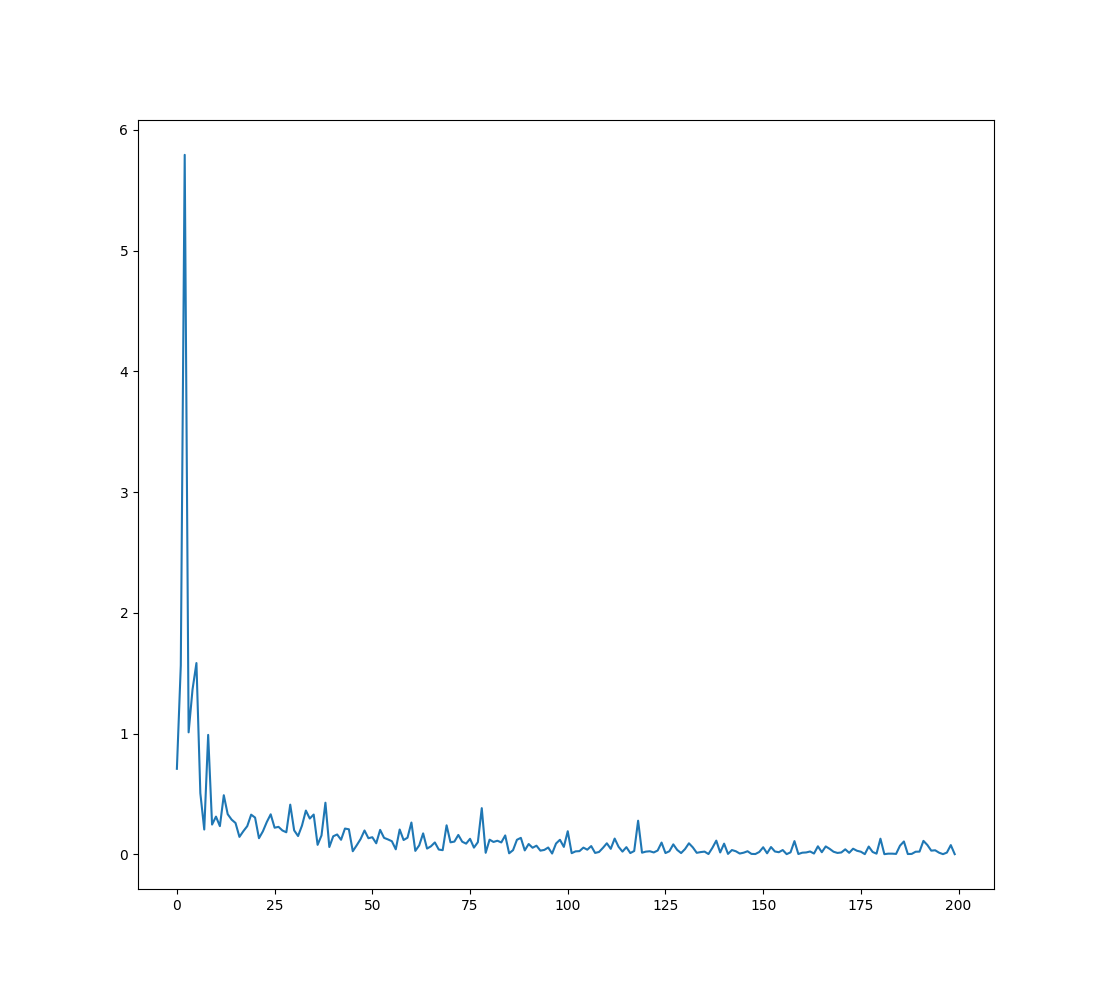
\includegraphics[width = 4.2in]{images/metrics.png}
	\centerline{\captionof{Figure 4.5: }{The model loss after incorporating Convolutional Layers}}
\label{good_metrics}
\end{center}


\begin{center}
	\centering
	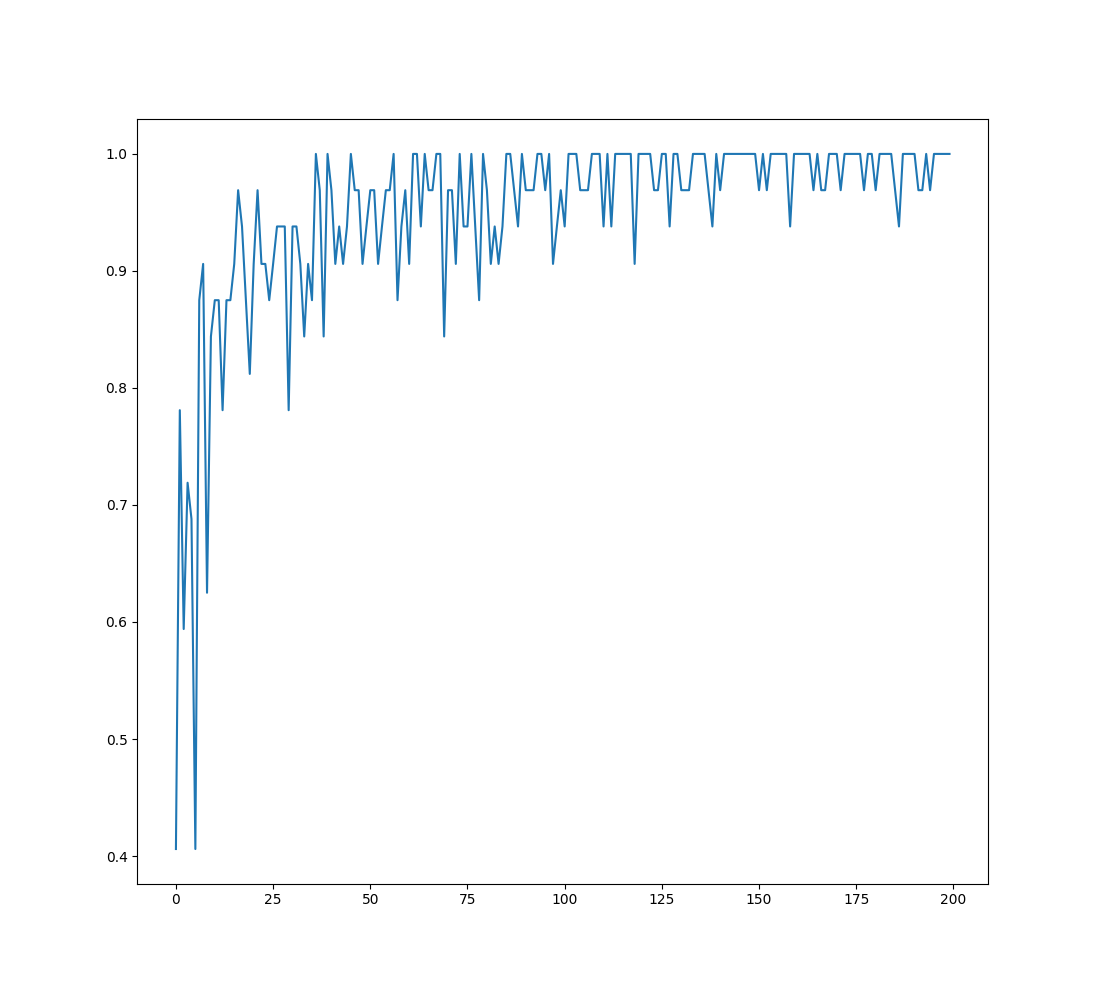
\includegraphics[width = 4.2in]{images/goodacc.png}
	\centerline{\captionof{Figure 4.6: }{The model accuracy after incorporating Convolutional Layers}}
\label{good_metrics2}
\end{center}

The general flow of the data in the Neural Network Framework is based on the forward-backward propagation principle,
specific to the \textit{Convolutional Neural Network} architecture.
Each of the trainable model's layers have the following methods:

\begin{enumerate}
	\item :function:forward(inputs): A method which takes the previous layer output as the parameter(inputs)
	and perform the specific operations, thus performing the forward data processing.
	\item :function:backward(derivated values): A method which takes the previous layer output, which consists
	of the gradient of the forward propagation end result(derivated values), performing the inverse
	computations in regards to the forward method, and then propagating the end result to the next layer.
	\item :parameter:output: A \textit{ndarray} where the \textit{forward} function computations are stored.
	\item :parameter:derivated input: A \textit{ndarray} where the \textit{backward} function computations are stored.

\end{enumerate}

The following diagram ilustrates the forward-backward propagation of the Neural Network Model.

\begin{center}
	\centering
	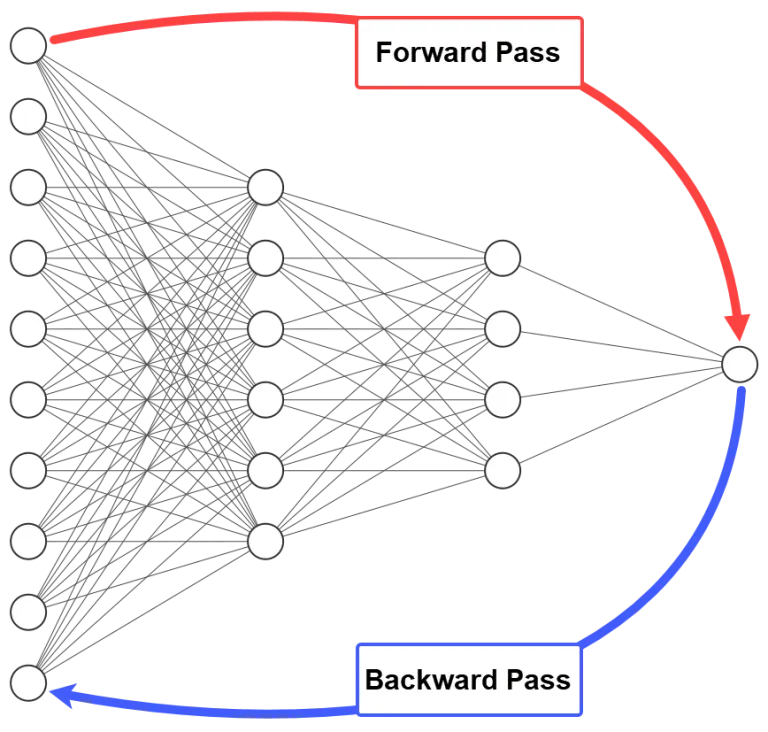
\includegraphics[width = 4.2in]{images/fwbw.png}
 \centerline{\captionof{Figure 4.7: }{Data flow throughout the model (image source \cite{fwbw})}}
\label{data_flow}
\end{center}

Because the model of the Neural Network Engine is effectively a Convolutional Neural Network, the training process follows
the following schema:


\begin{center}
	\centering
	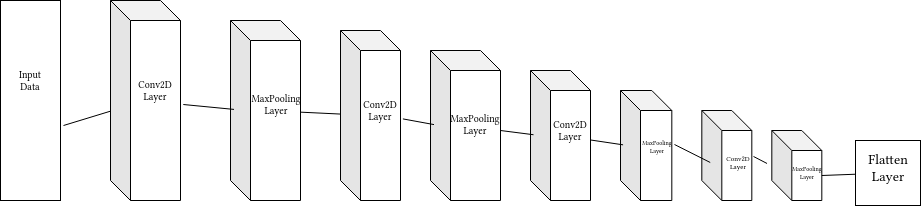
\includegraphics[width = 5.5in]{images/conv2d.png}
	\centerline{\captionof{Figure 4.8: Convolutional Neural Network architecture illustration. }}
\label{genarch}
\end{center}

At the end of each iteration the model has to classify unseen data ( the \textit{validation data}), and based on the results of
the classification, the model \textit{metrics} are computed, in the form of loss (computed with \textit{Categorical CrossEntropy})
and accuracy (computed with \textit{CategoricalAccuracy}).


\section{User Input Handling and Processing}

The modus operandi of the input handling and processing pipeline is presented in the following diagram.

\begin{figure}[H]
	\centering
	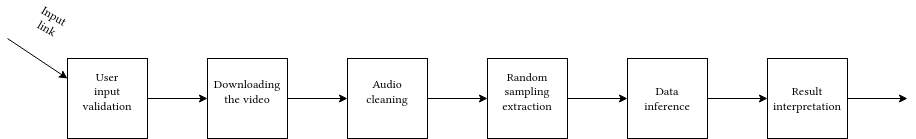
\includegraphics[width = 6.5in,height=1.3in]{images/datapipe.png}
	\centerline{\captionof{Figure 4.9: User input handling pipeline}}
\label{mo}
\end{figure}

The steps performed in order process the user input are as follows:
\begin{enumerate}

	\item Validating the user input : Checking if the input link inserted by the user is a valid YouTube link to
	either a video or a playlist.
	\item Downloading the video : Saving and converting the video at the specified link in a temporary folder.
		The \textit{youtube-dl} utilitary facilitates this step by downloading the file using
	a list of specified configuration parameters such as audio quality and the output format. After this step,
	we will have obtained an audio file of format wav in a temporary folder, which will be deleted after
	the finish of the prediction operation.
	\item Audio file cleaning: Given the reason that the model was trained on 1 second snippets of audio files of sample rate of 16000,
		the following operations are necessary to be performed to the audio file in order for it to be compatible with the Neural Network Engine:
		\begin{itemize}
			\item Downsampling the wav file to mono: Reducing the number of channels of the file to
			mono with the function \textit{to mono} from \textit{librosa}.
			\item Cleaning the wav file by sound envelope.
			\begin{figure}[H]
				\centering
				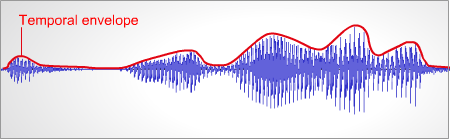
\includegraphics{images/soundenvelope.png}
				\centerline{\captionof{Figure 4.10: Sound envelope example (Source \cite{sev})}}
			\label{se}
			\end{figure}

	The sound envelope (presented in the figure \ref{se}), represents the changes in audio frequency over a period
	of time. The \textit{split wav by sound envelope} function computes a \textit{filtered mask} of the audio file
	by comparing each value of the sound envelope to a given threshold, thus eliminating the audio noise(such as
	crowd cheering and silence), keeping only the relevant audio information.

			\item Splitting the masked audio file: After the first two steps of the audio processing,
	the audio file has to be splitted into 1 second samples and converted to a sample rate of 16000.
		\end{itemize}

	\item Extracting a number of random sound samples: In order to offer an accurate prediction and reduce the
	time cost required by the Neural Network Engine, we randomly extract a number of samples from the splitted audio
	file.
\item Loading the random sound samples into the model: The Neural Network Engine also presents the \textit{inference}
	functionality. The inference/prediction is performed by transforming the input data (transformation performed
	by the input layer), then performing the forward-backward data propagation once.
	The transformations applied by the input layer are:
	\begin{itemize}

		\item Short Time Fourier Transformation

		Short Time Fourier Transformation is a mathematical transformation technique used for
		decomposing a function relative to its spatial and temporal dependencies. Since the audio signal is
		composed of sound wave which only ilustrate the amplitude of
		a recording, the Fourier transform allows for the creation of an illustration of a frequency
		over time,called spectrum. \cite{ft}

			\begin{figure}
				\centering
				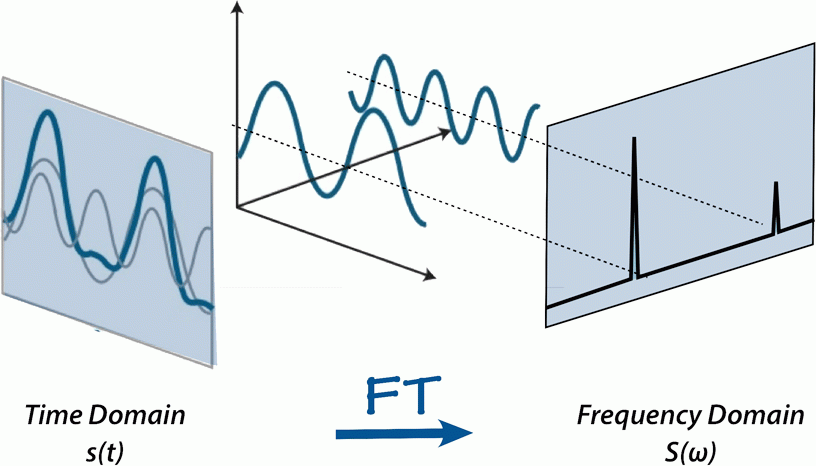
\includegraphics[width = 4.5in]{images/ft.png}
			\centerline{\captionof{Figure 4.11: Fourier transformation (Source \cite{ft})}}
			\label{ft}
			\end{figure}


		\item MEL Filterbank transformation

			The \textit{MEL} scale is a reprezentation of the sounds that can be heard and
			distinguished by the human ear. The \textit{MEL spectogram} is a graphical representation
			of the sound variations and intensities of the a given audio sample. With the
			\textit{MEL Filterbank transformation} we effectively represent the relevant information
			of the input data, thus transforming the problem from an audio classification
			into an image classification one.


			\begin{figure}[H]
				\centering
				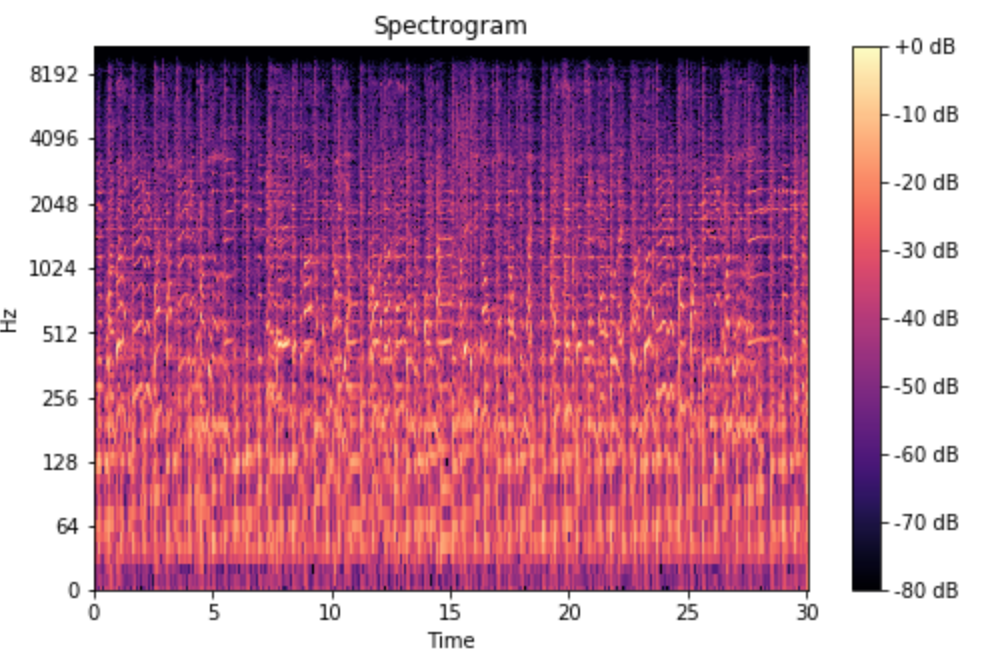
\includegraphics[width = 5.5in]{images/mel.png}
				\centerline{\captionof{Figure 4.12: MEL Spectogram example}}
			\label{ms}
			\end{figure}


	\end{itemize}



	The output of the transformation is a \textit{ndarray} containing the MEL spectogram
	of the input sample which represents the neural network model's input.\\
	The inference output is an array containing floating point numbers which represent the confidence
	value of the model prediction.\\
	The predicted label is computed by extracting the \textit{argmax}(the index
	of the element with the biggest value), then mapping it to the specific class name.


	\item Interpreting the result and returning the final prediction: The output label is stored for each prediction
	extracted from the random samples batch. The final label is computed by extracting the prediction
	which was suggested most often.

\end{enumerate}
\section{The Application-User Interaction}
	The application provides a minimalistic Graphic User Interface which offers the end user the means for
	classifying an YouTube song, as well as visualise the specific 3D Animation depending on the model prediction. \\
	In order to enrich the visual experience, we have choosen two 3D animations, projected using \textit{Autodesk Maya}.\\
	The main elements of the GUI are the textbox where the user inputs the link to the song, the submit
	button which grabs the link inserted by the user and begins the inference process and the video stream box,
	which appears after the model has performed the classification. The application runs over a \textit{main loop},
	meaning that the user can input as many links as desired in a session.


	The following figure illustrates some of the application states.


			\begin{center}
				\centering
				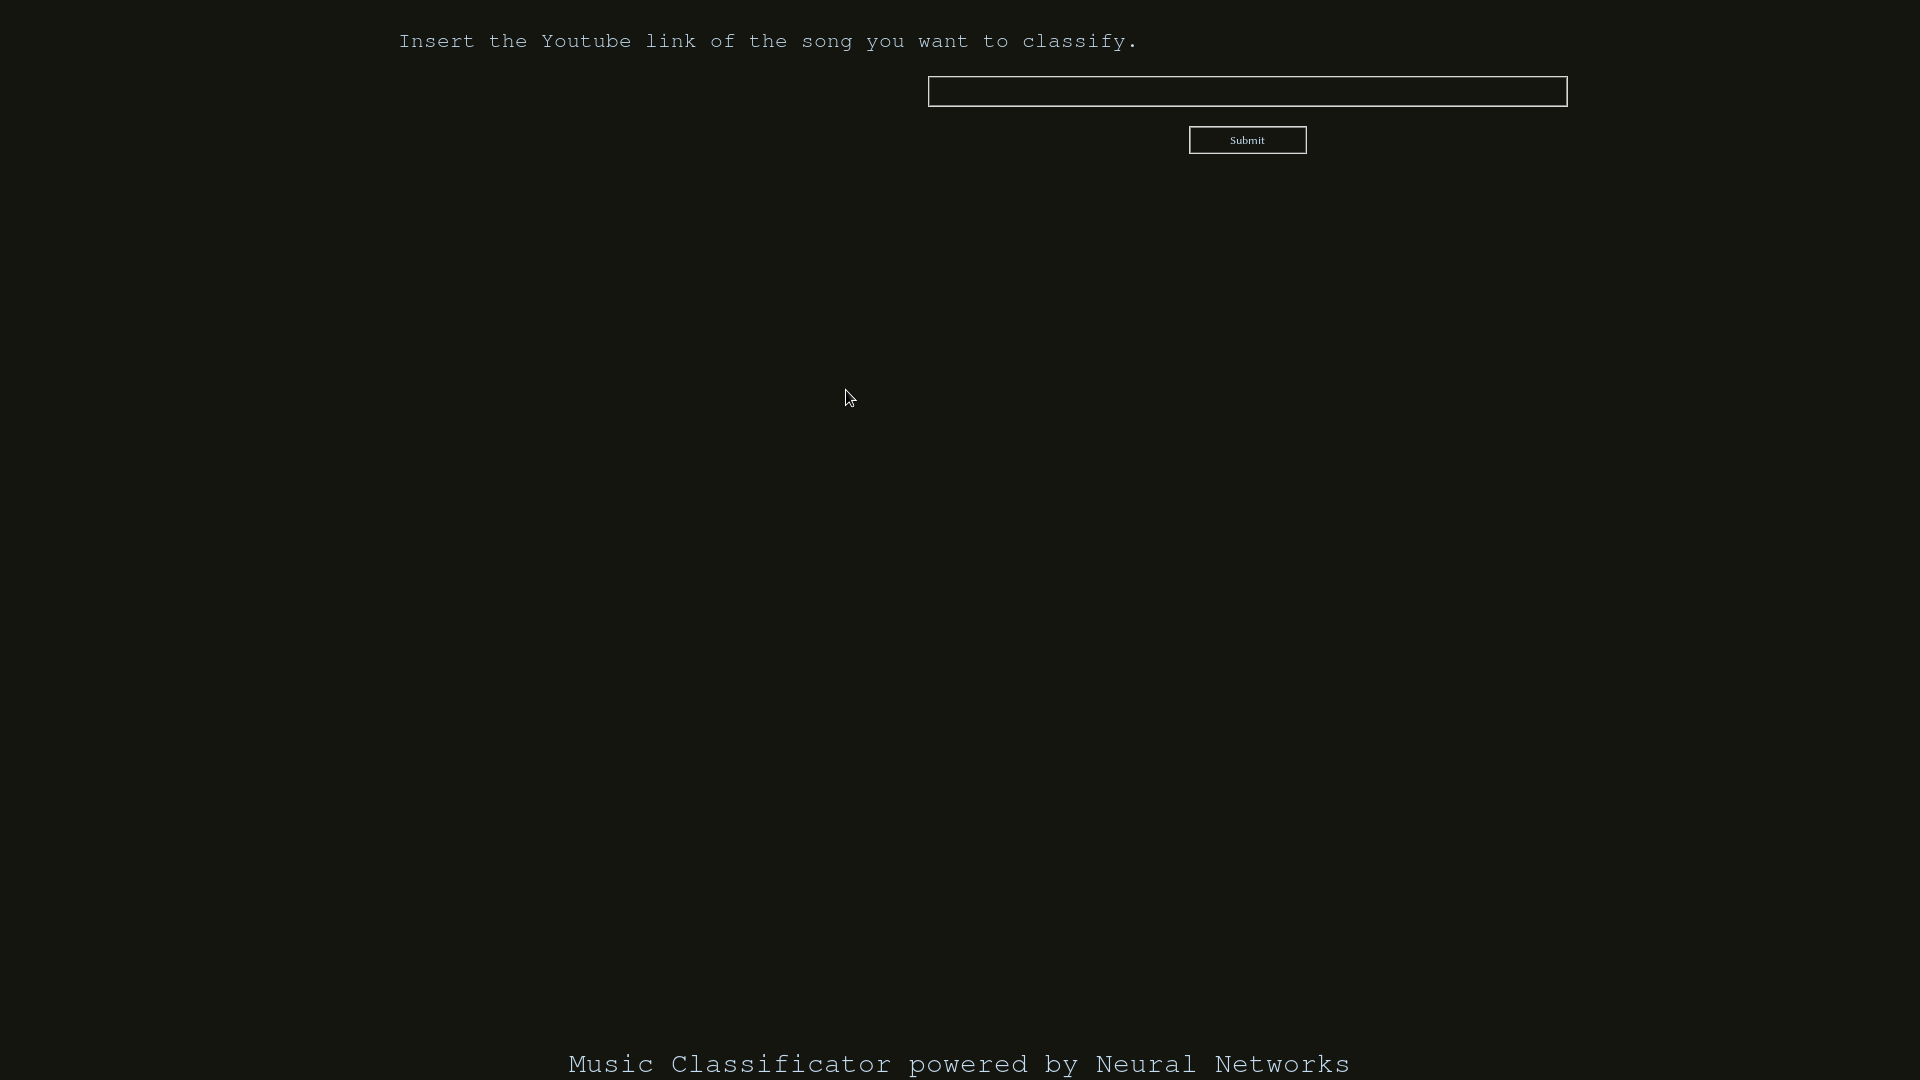
\includegraphics[width = 5.5in]{images/basic_interface.png}
				\centerline{\captionof{Figure 4.13: The Graphic User Interface at the start of the application.}}
			\label{guis}
			\end{center}

			\begin{center}
				\centering
				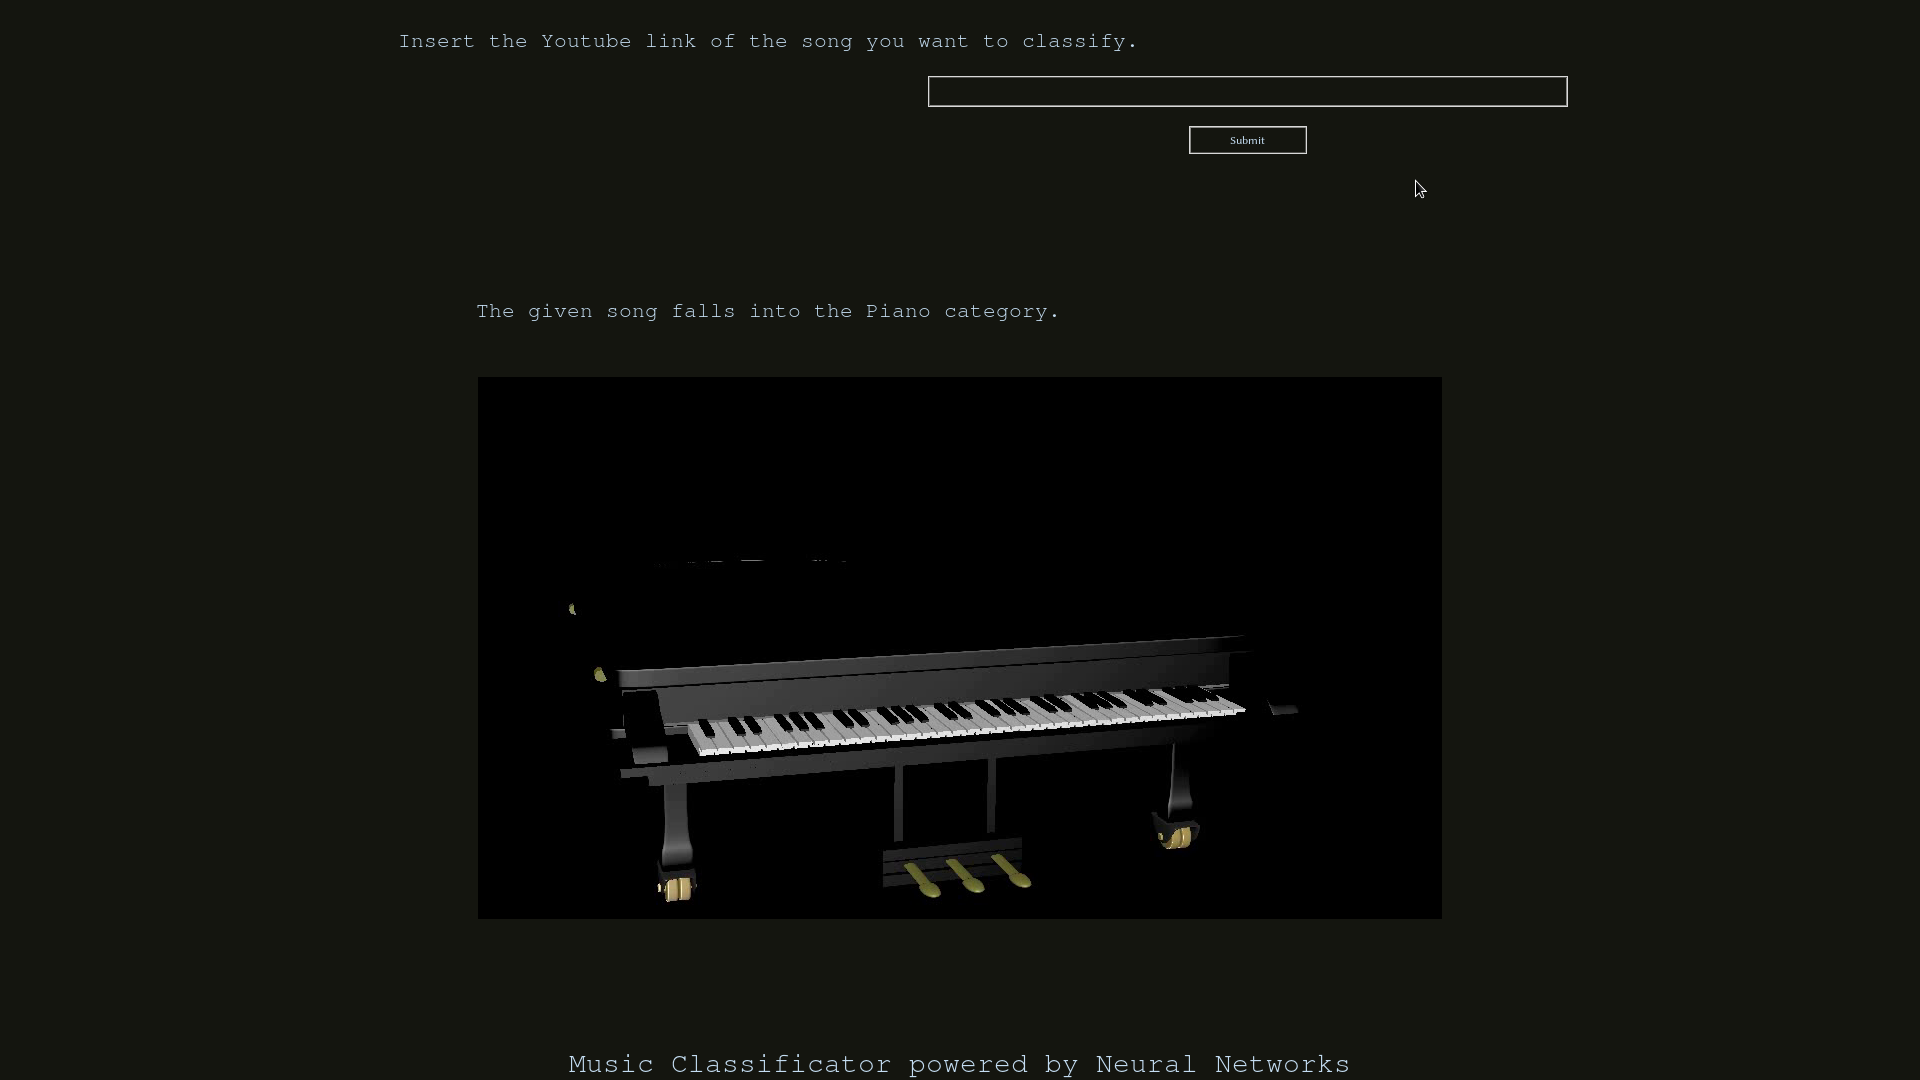
\includegraphics[width = 5.5in]{images/piano.png}
			\centerline{\captionof{Figure 4.14: The Graphic User Interface after predicting a song as a piano song.}}
			\label{guip}
			\end{center}

			\begin{center}
				\centering
				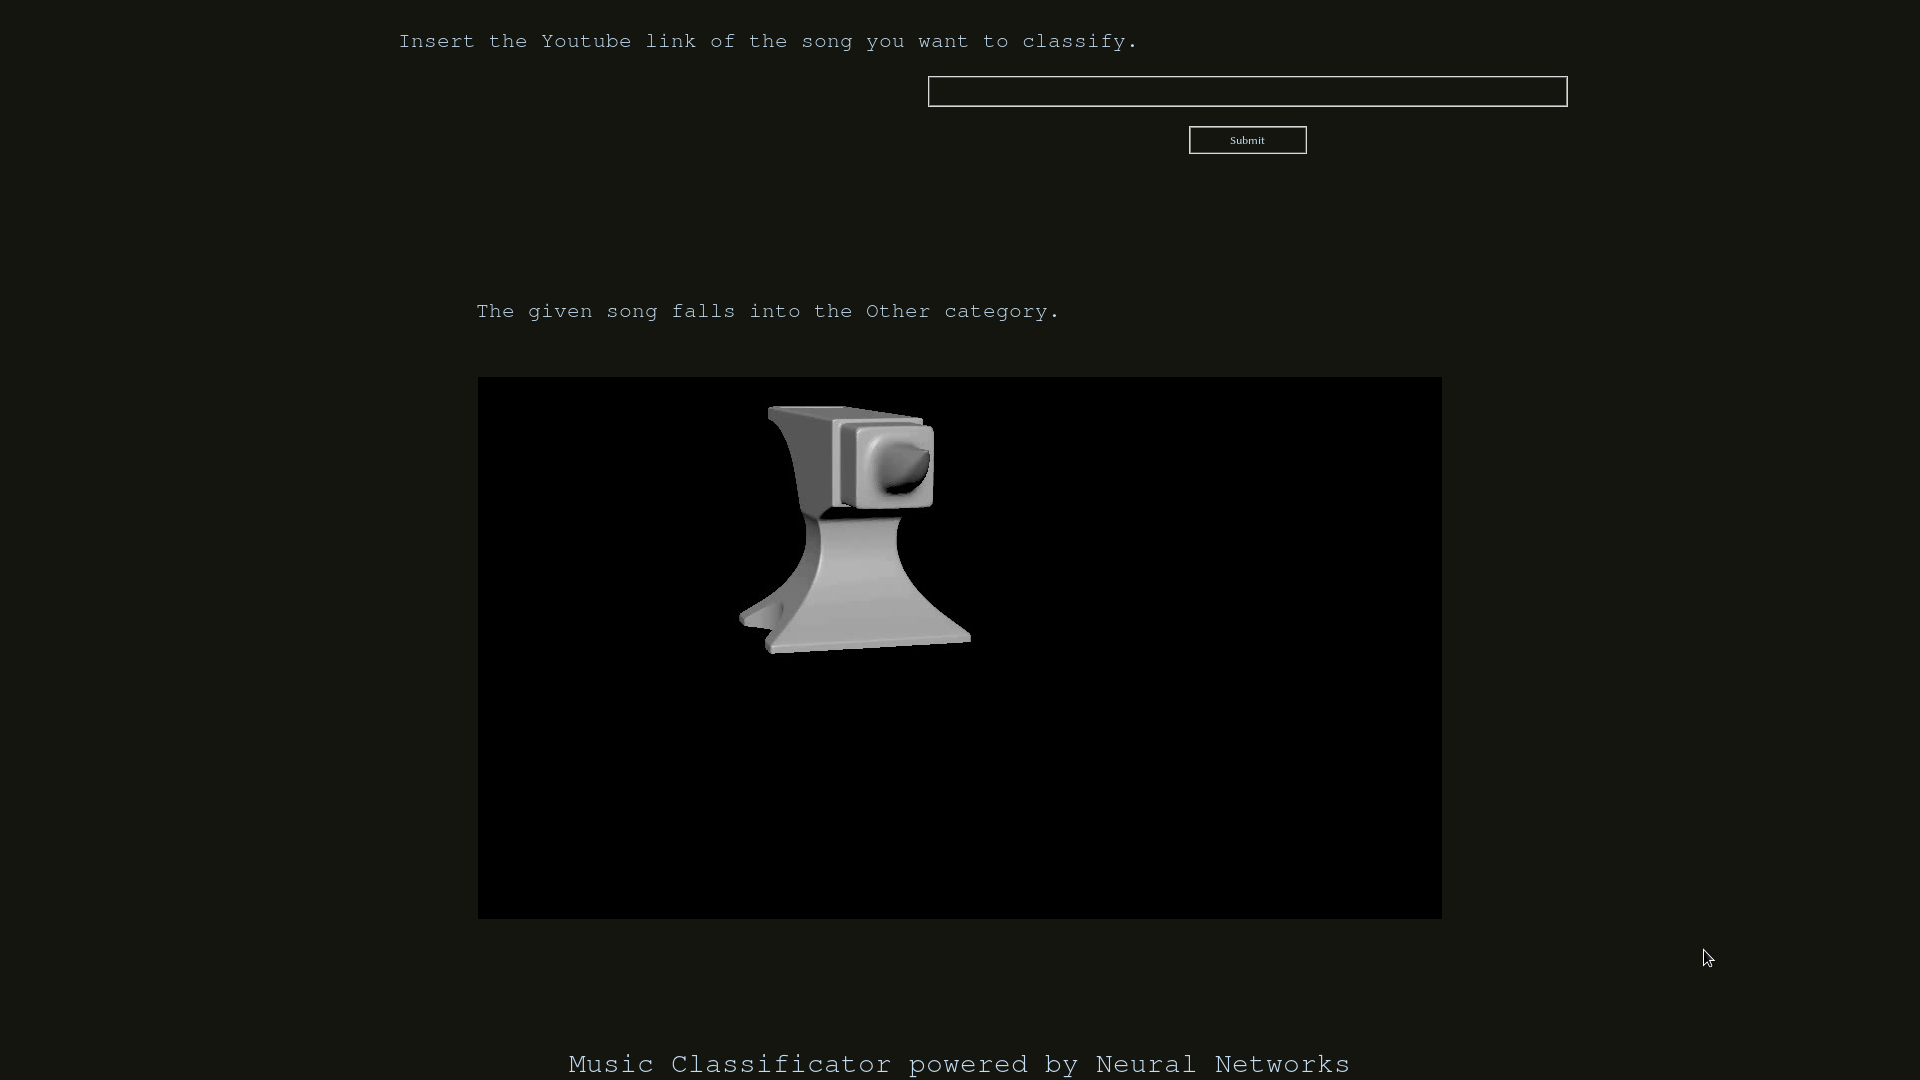
\includegraphics[width = 5.5in]{images/other.png}
				\centerline{\captionof{Figure 4.15: The Graphic User Interface after classifying a song as other.}}
			\label{guio}
			\end{center}
